%!iTeXMac(project): pdflatex
%! iTeXMac(mark): ADDED

\documentclass{acm-final/sig-alternate-modified}
\usepackage{parallel}

\newif\ifpdf
\ifx\pdfoutput\undefined
\pdffalse % we are not running PDFLaTeX
\else
\pdfoutput=1 % we are running PDFLaTeX
\pdftrue
\fi

\ifpdf
\usepackage[pdftex]{graphicx}
\else
\usepackage{graphicx}
\fi

% HC - Always use the EPS version
%\DeclareGraphicsExtensions{.eps}

\ifpdf
\DeclareGraphicsExtensions{.pdf, .jpg}
\else
\DeclareGraphicsExtensions{.eps, .jpg}
\fi

\newcommand{\stt}[1]{\scriptsize {\tt #1}}

\begin{document}

%\conferenceinfo{ICSOC'04,} {November 15--19, 2004, New York, New York, USA.}  
%\CopyrightYear{2004}  
%\crdata{1-58113-871-7/04/0011}


\title{llava - Java in Lisp Syntax}

\numberofauthors{1}

\author{
\alignauthor Harold Carr \\
       \email{carr@llava.org}
}

\toappearbox{Submitted to the International Lisp Conference 2005}

\maketitle

%======================================================================
\begin{abstract}

{\tt llava} is Java in Lisp (lack of) syntax (rather than a Lisp or
Scheme written in Java).  {\tt llava} does not contain special syntax
or functions to call Java methods nor does it define an orthogonal set
of types (such as Scheme strings or Common Lisp arrays).  Instead,
{\tt llava} is Java expressed in typical prefix list syntax with all
data being native Java data types (e.g., instances of Java classes).
{\tt llava} adds additional types (e.g., {\tt Pair}, {\tt Procedure},
{\tt Symbol} and {\tt Syntax}) to enable one to work with lists and to
define procedures and macros.

This paper discusses the motivation for Java, presents how it differs
from similar efforts, and describes its implementation: the
Reflective Invocation system that is the core of enabling {\tt llava}
to provide a prefix notation for Java method calls; how {\tt llava}
procedures (e.g., lambda) are integrated with Java such that method
invocations on Java objects take precedence over {\tt llava}
procedures; and extending {\tt package} and {\tt import} to work with
both Java class files and {\tt llava} procedures and files; and
finally, the {\tt llava} compilation strategy and the ``engine''-based
runtime.

\end{abstract}

%======================================================================

%\category{C.2.4}{Computer-Communication Networks}{Distributed Systems}
%\category{D.2.11}{Software Engineering}{Software Architectures}[patterns - remoting]

%\terms{Design}

\keywords{Lisp, Scheme, Java, Reflection, Modules}

%======================================================================
\section{Overview}

%======================================================================
\subsection{Motivation}

I once built Lisp systems \cite{LaSC5,LaSC3}.  Then funding caused me
to do C++ \cite{DC++}.  Then Java arrived and programming felt fun
again.  It reminded me I wanted more.  So I used Kawa \cite{kawa} for
interactivity and abstractions (i.e., macros).  But I kept running
into missing Scheme library items.  So I made foreign-function calls
to Java.  However, I had to convert between Kawa/Scheme I/O, strings,
characters, etc., and Java types.  (Note: this was with an early
version of Kawa.)  This lack of interoperability made me realize I
didn't want Lisp/Scheme in Java.

That's when I got the idea for {\tt llava}.  Why not create a version
of Java that uses Lisp syntax to write Java classes?  Then extend that
system to include a few special forms (e.g., {\tt lambda}, {\tt set!},
{\tt if}, {\tt quote}, {\tt define-syntax}), pairs and symbols, a REPL
and support for incremental (re)definition.

{\tt llava} \emph{is} access to Java via Lisp syntax and features.
The philosophy of {\tt llava} is: maximum leverage of Java---only add
what is missing or cannot be done in Java.

%======================================================================
\subsection{The llava language}
\label{the-llava-language}

{\tt llava} is a prefix version of Java expressed in list structure.
As such, it is \emph{not} a version of Scheme with special notation to
access Java (like Jscheme \cite{JschemeDot}) or a version of Common Lisp
with a foreign-function interface to Java (like ArmedBear Common Lisp
(ABCL) \cite{abcl}).  Table~\ref{j-l-j-a} compares language features
between Java, {\tt llava} and these other languages.  The table should
make it clear that {\tt llava} is a more direct prefix/list notation
of Java - {\tt llava}'s primary goal.

\begin{table*}
\centering
\caption{Notation Comparisons}
\begin{tabular}{|l|l|l|l|} \hline
Java		&	{\tt llava}	&	jscheme	& abcl \\ \hline

{\bf new} & & & \\ 

{\stt import java.util.Hashtable;}
                &{\stt (import java.util.Hashtable)}
                                        &{\stt (import "java.util.Hashtable")}
                                                        & \\
{\stt Hashtable ht = new Hashtable();}
                &{\stt (set! ht (new 'Hashtable))}
                                        &{\stt (set! ht (Hashtable.))}
                                            &{\stt (setq ht } \\
                &                       &   &\hspace{0.5em}{\stt   (jnew (jconstructor "java.util.Hashtable")))} \\

{\bf virtual method calls} & & & \\

{\stt ht.put("three", 3);}
                &{\stt (put ht "three" 3)}
                                        &{\stt (.put ht "three" 3)}

   &{\stt (jcall (jmethod "java.util.Hashtable" "put"} \\
&&&\hspace{2em} {\stt "java.lang.Object" "java.lang.Object")} \\
&&&\hspace{1em} {\stt ht "three" 3)} \\

{\bf static method calls} & & & \\

                &{\stt (import java.lang.Byte)}
                                        &
                                                     & \\
{\stt Byte b = Byte.decode("3");}
                &{\stt (set! b (Byte.decode "3"))}
                                    &{\stt (set! b (Byte.decode "3"))}
          &{\stt (setq b (jstatic } \\
 &&&\hspace{2em}{\stt (jmethod "java.lang.Byte" "decode"} \\
 &&&\hspace{2.5em}{\stt "java.lang.String")} \\
 &&&\hspace{1em}{\stt nil "3"))} \\ \hline

\end{tabular}
\label{j-l-j-a}
\end{table*}


Jscheme uses ``dot'' notation \cite{JschemeDot}.  This seems to have
one advantage over {\tt llava}: accessing a static field can be
accessed as a variable reference, whereas {\tt llava} chooses to
represent this as a procedure call.  Table~\ref{j-l-j} shows this
(along with virtual field access).

\begin{table*}
\centering
\caption{More Notation Comparisons}
\begin{tabular}{|l|l|l|} \hline
Java		&	{\tt llava}	&	jscheme	\\ \hline

{\bf virtual fields} & & \\

{\stt import org.omg.CORBA.IntHolder;}
                &{\stt (import org.omg.CORBA.IntHolder)}
  					&{\stt (import "org.omg.CORBA.IntHolder")} \\
{\stt IntHolder ih = new IntHolder();}
		&{\stt (set! ih (new 'IntHolder))}
					&{\stt (set! ih (IntHolder.))} \\
{\stt ih.value = 3;}
		&{\stt (value! ih 3)}
					&{\stt (.value\$ ih 3)} \\
{\stt ih.value;}
		&{\stt (value ih)}
					&{\stt (.value\$ ih)} \\
&&\\
{\bf static fields} & & \\

{\stt import java.io.File;}
		&{\stt (import java.io.File)}
					&{\stt (import "java.io.File")} \\
{\stt File.pathSeparator;}
		&{\stt (File.pathSeparator)}
					&{\stt File.pathSeparator\$} \\ \hline

\end{tabular}
\label{j-l-j}
\end{table*}

{\tt llava} presents Java directly (e.g., {\tt true} and {\tt false}
rather than Jscheme's {\tt \#t} and {\tt \#f}).  Along these lines,
rather than invent new module and condition systems, {\tt llava}
exposes {\tt package/import} and {\tt try/catch/finally} in a natural
way:



\small
\begin{verbatim}
(package org.llava.demo)

(import java.lang.ArithmeticException)
(import java.lang.Exception)

(let ((bomb 1))
  (define (demo)
    (try
       (if (< bomb 0)
           (throw (new 'Exception "Give up!")))
       (list "Normal result is: " (/ 2 bomb))
     (catch (ArithmeticException e)
       (list "Arithmetic: " e))
     (catch (Exception e)
       (list "Exception: " e))
     (finally
       (set! bomb (- bomb 1))))))
\end{verbatim}
\normalsize

%======================================================================
\subsection{Implementation}

%==================================================
\subsubsection{Reflective invocation}

{\tt llava}'s Reflective Invocation (RI) system enables access to Java
without special syntax or explicit foreign-function interfaces.  Once
a Java object is obtained its methods and fields are immediately
available:

\small
\begin{verbatim}
(toLowerCase (substring "Foo-Bar" 4))
  => "bar"
\end{verbatim}
\normalsize

{\tt llava} looks up {\tt llava} procedure definitions in internal
symbol tables.  If a procedure is \emph{not} defined then control goes
to the RI.  The RI uses Java reflection to invoke the appropriate
method by using the procedure call name as the method name, the first
argument as the class type (and message recipient) and the types of
the remaining arguments.

%==================================================
\subsubsection{llava procedures viz Java method calls}

A {\tt llava} procedure with the same name as a method of the first
argument (and matching argument types) will be invoked if defined with
an explicit {\tt lambda} as:

\small
\begin{verbatim}
(define toLowerCase
  (lambda (x) (toUpperCase x)))

(toLowerCase (substring "Foo-Bar" 4))
  => "BAR"
\end{verbatim}
\normalsize

Most of the time that is \emph{not} what you want to happen.  {\tt
llava} provides an alternate form of {\tt define} that allows Java
methods to take precedence:

\small
\begin{verbatim}
(define (toLowerCase x)
  (- x))

(toLowerCase (substring "Foo-Bar" 4))
  => "bar"
(toLowerCase 3.4)
  => -3.4
\end{verbatim}
\normalsize

In other words, if the lookup finds a procedure defined with an
explicit {\tt lambda} then that procedure will always be invoked
regardless of the argument types.  If lookup finds a procedure defined
\emph{without} an explicit {\tt lambda} then {\tt llava} will first
attempt an RI invocation.  If RI finds a method, it will invoke the
method and return the results.  If RI does not find a method then the
{\tt llava} procedure will be invoked.  If lookup does not find either
type of {\tt llava} procedure then {\tt llava} will throw a {\tt
LlavaException} indicating an undefined top-level variable.

%==================================================
\subsubsection{package/import system}

Like Java, {\tt llava}'s {\tt import} enables ``short''-form access to
constructors and static methods and static fields:

\small
\begin{verbatim}
(import java.lang.Long)
(set! l (new 'Long 34))
(getName (getClass (Long.decode "23")))
 => "java.lang.Long"
(Long.MAX_VALUE)
 => 9223372036854775807

(import java.lang.System)
(System.out)
 => java.io.PrintStream@1434234
\end{verbatim}
\normalsize

When a Java class is imported, {\tt llava} creates a {\tt llava}
package for that class and defines procedures in that package to
access fields.  It also adds the imported package to the list of
packages imported by the package doing the importing.  Then, during
variable lookup, any names with a single dot (``.'') in them will be
expanded to the full package name.

% What about foo.bar.inner to get inner classes?

{\tt llava} code may define packages:

\small
\begin{verbatim}
(package org.example)

(define (whatZone x)
  (let* ((tz (getTimeZone x))
         (n  (getDisplayName tz)))
    n))
\end{verbatim}
\normalsize

%(whatZone (DateFormat.getInstance))

Details of {\tt llava}'s {\tt package} and {\tt import} implementation
and how they interact with Java {\tt classpath}, the file system, and
the REPL are given in the main body of the paper.


%==================================================
\subsubsection{Compiler and runtime system}

{\tt llava} is compiled to a few special forms: application, {\tt
begin}, {\tt if}, {\tt lambda}, literal, ref, {\tt set!}.  Those forms
are written as explicit Java classes, each with a {\tt run} method
that takes the current lexical environment and an evaluation engine
that also has a {\tt run method}.  The forms and the engine cooperate
such that the same call to {\tt engine.run} is executed in a Java {\tt
while} loop when evaluating tail calls.  This makes the {\tt llava}
interface to Java properly tail-recursive.  The engine evaluator is
similar to one used in older versions of Jscheme \cite{JschemeEngine}.

%==================================================
\subsection{Contribution}

The main contribution of {\tt llava} is that it is Java in Lisp syntax
rather than another language written in Java.  It extends Java by
providing macros, procedures, lists, and symbols.  Its core feature is
automatic Reflective Invocation enabling method calls on Java objects
without special syntax, declarations or APIs.

Another contribution is the {\tt package/import} algorithm for
enabling dynamic hierarchies of namespaces for top-level variables.

The remainder of this paper gives more details on the design of the
language, implementation techniques and performance.

%======================================================================
\section{The llava language}

The examples shown so far have emphasized defining and calling {\tt
llava} procedures as well as creating Java objects and calling methods
on those objects.  {\tt llava}'s automatic RI system enables both
types of calls to look the same.  This, coupled with support for {\tt
try}, {\tt throw}, {\tt synchronized}, etc., enables one to write
procedures in a prefix form of Java.

It is also desirable to write interface and class definitions directly
in {\tt llava}.  Table~\ref{definingClasses} shows an extended working
example of defining and inheriting (abstract) classes in Java and the
equivalent {\tt llava} code.  The symmetry between both versions
derives from {\tt llava}'s goal to be Java in Lisp syntax.  Rather
than devise a new notation for defining classes, {\tt llava} provides
an intuitive ``lispy'' syntax such that the mental translation
required to move between Java or {\tt llava} syntax is reduced.

\begin{table*}
\caption{Defining Classes}
%\tiny
%\scriptsize
%\footnotesize
%\small
%\normalsize
{\footnotesize

\begin{Parallel}{0.4\textwidth}{0.4\textwidth}

%%%%%%%%%%%%%% PointBase

  \ParallelPar
  \ParallelLText{{\bf org/llava/pb/PointBase.java}}
  \ParallelRText{{\bf org/llava/pb/PointBase.lva}}

  \ParallelPar
  \ParallelLText{\begin{verbatim}

package org.llava.pb;

import java.util.LinkedList;
import java.util.List;

public abstract class PointBase {
    protected List history = new LinkedList();
    protected int x = 0;
    protected int y = 0;
    public int getX() { return x; }
    public int getY() { return y; }
    protected void move(int dx, int dy) {
        x += dx; y += dy; moved();
    }
    protected void moved() {
        history.add(this.toString());
        System.out.println("Moved: " + this);
    }
    public List getHistory() { return history; }
    public String toString() {
        return getName() + " x: " + x + " y: " + y;
    }
    protected abstract String getName();
}\end{verbatim}}
  \ParallelRText{\begin{verbatim}(package org.llava.pb)

(import java.util.LinkedList)
(import java.util.List)

(public abstract class PointBase
  (protected List history (new 'LinkedList))
  (protected int x 0)
  (protected int y 0)
  (public int (getX) x)
  (public int (getY) y)
  (protected void (move dx dy)
    (+= x dx) (+= y dy) (moved this))

  (protected void (moved)
    (add history (toString this))
    (println (System.out) (+ "Moved: " this))

  (public List (getHistory) history)
  (public String (toString)
    (+ (getName) " x: " x " y: " y))

  (protected abstract String (getName)))\end{verbatim}}

%%%%%%%%%%%%%% ColoredPointBase

  \ParallelPar
  \ParallelLText{{\bf org/llava/pb/ColoredPointBase.java}}
  \ParallelRText{{\bf org/llava/pb/ColoredPointBase.lva}}

  \ParallelPar
  \ParallelLText{\begin{verbatim}package org.llava.cp;

import org.llava.pb.PointBase;

public abstract class ColoredPointBase 
    extends PointBase {
    protected String color;
}\end{verbatim}}
  \ParallelRText{\begin{verbatim}(package org.llava.cp)

(import org.llava.pb.PointBase)

(public abstract class ColoredPointBase 
  extends PointBase
  (protected String color))\end{verbatim}}

%%%%%%%%%%%%%% Point

  \ParallelPar
  \ParallelLText{{\bf org/llava/pb/Point.java}}
  \ParallelRText{{\bf org/llava/pb/Point.lva}}

  \ParallelPar
  \ParallelLText{\begin{verbatim}package org.llava.p;

import org.llava.pb.PointBase;

public class Point extends PointBase {
    protected String getName() {
        return getClass().getName();
    }
}\end{verbatim}}
  \ParallelRText{\begin{verbatim}(package org.llava.p)

(import org.llava.pb.PointBase)

(public class Point extends PointBase
  (protected String (getName)
    (getName (getClass this))))\end{verbatim}}

%%%%%%%%%%%%%% ColoredPoint

  \ParallelPar
  \ParallelLText{{\bf org/llava/pb/ColoredPoint.java}}
  \ParallelRText{{\bf org/llava/pb/ColoredPoint.lva}}

  \ParallelPar
  \ParallelLText{\begin{verbatim}package org.llava.cp;

import org.llava.cp.ColoredPointBase;

public class ColoredPoint 
    extends ColoredPointBase {
    public ColoredPoint(String color) {
        this.color = color;
    }
    protected String getName() {
        return getClass().getName()
            + " color: " + color + " ";
    }
}\end{verbatim}}
  \ParallelRText{\begin{verbatim}(package org.llava.cp)

(import org.llava.cp.ColoredPointBase)

(public class ColoredPoint 
  extends ColoredPointBase
  (public (ColoredPoint (String c))
    (= color c))

  (protected String (getName)
    (+ (getName (getClass this))
       " color: " color " ")))\end{verbatim}}

%%%%%%%%%%%%%% ThreeDPoint

  \ParallelPar
  \ParallelLText{{\bf org/llava/pb/ThreeDPoint.java}}
  \ParallelRText{{\bf org/llava/pb/ThreeDPoint.lva}}

  \ParallelPar
  \ParallelLText{\begin{verbatim}package org.llava.tdp;

import org.llava.p.Point;

public class ThreeDPoint extends Point {
    protected int z = 0;
    public int getZ() { return z; }
    protected void move(int dx, int dy, int dz) {
        z += dz;
        move(dx, dy);
    }
    public String toString() {
        return super.toString() + " z: " + z;
    }
}\end{verbatim}}
  \ParallelRText{\begin{verbatim}(package org.llava.tdp)

(import org.llava.p.Point)

(public class ThreeDPoint extends Point
  (protected int z 0)
  (public int (getZ) z)
  (protected void (move dx dy dz)
    (+= z dz)
    (move this dx dy))

  (public String (toString)
    (+ (toString super) " z: " z)))\end{verbatim}}
\end{Parallel}
}
\label{definingClasses}
\end{table*}

%======================================================================
\subsection{llava language design}

It may seem that {\tt llava}'s notation for classes is simple.
However, the apparent simplicity is the result of numerous small
design decisions.

%=================================
\subsubsection{Methods and fields}

Referring to {\tt PointBase} in Table~\ref{definingClasses}, note that
a choice has been made in representing fields and methods.  The field:

\small
\begin{verbatim}
    protected int x = 0;
\end{verbatim}
\normalsize

could have been represented in many ways.  The final two candidates
were:

\small
\begin{verbatim}
    (protected x 0)
    (protected int x 0)
\end{verbatim}
\normalsize

The first form was initially considered since type declarations are
not necessary in {\tt llava}.  However, if methods on classes defined
in {\tt llava} are to be called from Java then it is useful to have
type information.

Similarly, method representation had several candidates:

\small
\begin{verbatim}
    (public     getX() (return x))
    (public int getX() (return x))
    (public int getX() x)
    (public int (getX) x)
\end{verbatim}
\normalsize

The declaration of the return type could be omitted, but like fields,
it is useful to have that information when calling from Java.  Also,
keeping field types and method return types keeps {\tt llava}
representation closer to Java, thereby easing the translation burden.
Since all forms in {\tt llava} are expressions there is no need for a
{\tt return} statement ({\tt llava}'s {\tt call/ep} can be used for
the cases where a {\tt return} is needed.  {\tt call/ep} provides
continuations with dynamic extent \cite{queinnec}).  Finally, since
{\tt llava} defines procedures using Scheme syntax it was decided to
be consistent and include the method name at the head of the list of
arguments.  This also makes it easier to distinguish between fields
and methods when parsing class defined in {\tt llava}.

The previous sentence points out conflicting constraints in the design
of {\tt llava}: stay close to a prefix version of Java while borrowing
features from Lisp (i.e., Scheme).  To settle a design issue it is
useful to keep in mind the target user of {\tt llava} (besides the
author).  Perhaps a prefix version of Java will hit a sweet spot,
resulting in bringing programmers to Lisp, much in the same way Java's
similarity with C/C++ enabled C/C++ programmers to more easily migrate
to Java.  But programmers fluent in Lisp may prefer to have well-known
Lisp patterns available.  The tension of these conflicting constraints
is seen at every step in the design of the {\tt llava} language.

%=================================
\subsubsection{Lexical structure}

There are many possibilities in representing Java comments:

\small
\begin{verbatim}
    // single line comment
    ;  ...

    /* block
       comment */
    (/* ...)
    (-comment- ...)

    /**
     * @author me
     */
    (/** @author)
    (-doc- ...)
\end{verbatim}
\normalsize

At present {\tt llava} uses {\tt ;}, {\tt -comment-} and {\tt -doc-}.
However, {\tt llava} is moving towards settling all language design
issues in favor of Java.  Therefore support for {\tt //}, {\tt /*} and
{\tt /**} seems likely.  Using direct Java style block and javadoc
comments requires more lexical processing since {\tt read} (and
macros) cannot be used to do the work.  Using a prefix version of Java
style block and javadoc comments seems like a good solution but it is
easy to trip {\tt read} up:

\small
\begin{verbatim}
    (/* more . . .)
\end{verbatim}
\normalsize

That example will cause {\tt read} to fail looking for the end of a
cons cell.  Perhaps a compromise to keep the implementation simple while leaning
toward Java is to use strings inside of comments:

\small
\begin{verbatim}
    (/* "more . . .")
\end{verbatim}
\normalsize

%=================================
\paragraph{Identifiers}

When defining procedures and local variables {\tt llava} supports
``Lispy'' characters:

\small
\begin{verbatim}
(define *global* 3)
(define (some-procedure 1st-arg 2nd-arg)
  (let ((+sum+ (+ 1st-arg 2nd-arg)))
    (list +sum+ *global* '-foo)))
\end{verbatim}
\normalsize

Identifiers for interfaces, classes, fields and methods must follow
Java rules.

%=================================
\paragraph{Literals}

{\tt llava} reserves Java keywords such as {\tt public}, {\tt
abstract} and {\tt static} and adds a number from Lisp such as {\tt
define}, {\tt defmacro}, {\tt lambda}, {\tt quote} and {\tt let}.
Boolean literals are {\tt true false} rather than {\tt \#t \#f} or
{\tt t nil}.

Even though {\tt llava} tries to settle design decisions in favor of
Java there are some cases where Lisp clearly wins out, such as
character representation.  Java specifies characters as {\tt 'a'} but
the {\tt quote} reader macro is so fundamental to Lisp history that it
cannot be used for characters.  In this case {\tt llava} uses the Lisp
representation: \verb+#\a+.

%=================================
\paragraph{Operators}

Built-in operators are a place that brings the conflicting constraints
to the fore:

\small
\begin{tabular}{l|l|l}
\verb+foo = bar;+        & \verb+(= foo bar)+      & \verb+(set! foo bar)+ \\
\verb+x == y+            & \verb+(== x y)+         & \verb+(eq? x y)+ \\
\verb+x && y+            & \verb+(&& x y)+         & \verb+(and x y)+ \\
\verb+x != y+            & \verb+(!= x y)+         & \verb+(not (eq? x y))+ \\
\verb+!x+                & \verb+(! x)+            & \verb+(not x)+ \\
\verb%x += 1%            & \verb%(+= x 1)%         & \verb%(set! x (+ x 1))%\\
\end{tabular}
\normalsize

At present {\tt llava} uses the Scheme versions.  However it seems
advisable to change and favor the prefix Java versions, not only to
provide an intuitive translation for non-Lisp/Scheme programmers, but
to avoid shadowing valid method names such as {\tt and} and {\tt not}.

%=================================
\subsubsection{Types, values and variables}

{\tt llava}'s RI system does autoboxing of primitive types.  Variables
in {\tt llava} interfaces and classes can have modifiers and/or types.
Table~\ref{definingClasses} shows modified and typed fields and return
types of methods.  {\tt llava} also supports specifying the types of
method parameters:

\small
\begin{verbatim}
(import java.util.Hashtable)
(import java.util.Map)

(public class Table
  (private static int numCreated 0)
  (private Map table)

  (public (Table)
    (+= numCreated 1)
    (= table (new 'Hashtable)))

  (public static int (numCreated)
    numCreated)

  (public void (put (String key) (int value))
    (put table key value))

  (public int (get (String key)) 
      throws NoSuchElementException
             MinusOneException
    (let ((v (get table key)))
      (cond ((== v null)
             (throw (new 'NoSuchElementException)))
            ((< v 0)
             (throw (new 'MinusOneException)))
            (else
             (intValue v))))))
\end{verbatim}
\normalsize

Note that {\tt llava} does not support modifiers or types in {\tt
llava} procedure variables and local variables.

%=================================
\subsubsection{Inheritance and declaring exceptions}

The previous example has a method {\tt get} declaring checked
exceptions.  To someone used to Lisp, the declaration seems to be
``floating''---to be missing parenthesis.  Perhaps it would be better
as:

\small
\begin{verbatim}
  (public int (get (String key)) 
      (throws NoSuchElementException
              MinusOneException)
    ...)
\end{verbatim}
\normalsize

However, for consistency, that would require changing the notation for
inheritance in Table~\ref{definingClasses} to:

\small
\begin{verbatim}
(public class Point (extends PointBase)
  ...)
\end{verbatim}
\normalsize

{\tt llava} currently supports the non-parenthesized version.

%=================================
\subsubsection{Blocks, statements and expressions}

Local variables and blocks are introduced with {\tt let} and {\tt
begin}.  As shown in a previous example
(Section~\ref{the-llava-language}, {\tt llava} provides {\tt
try/catch/finally}.  All {\tt llava} statements are expressions that
return values.

%=================================
\paragraph{Looping}

{\tt llava} supports last-call-optimization for procedures so
recursion is encouraged.  However, when calling methods on classes
defined with {\tt llava}, recursion is discouraged since the method
calls go through Java's call stack.  {\tt llava}'s {\tt while} macro
may be used instead.  {\tt do} in {\tt llava} is Lisp's {\tt do}
rather than Java's {\tt do/while}.

The only abrupt transfer of control supported by {\tt llava} is {\tt
throw} as shown in the {\tt Table} example above.  {\tt call/ep} can
be used where {\tt break continue} and {\tt return} are needed.

%=================================
\subsubsection{Anonymous classes}

The syntax for an anonymous Java class is quite cumbersome:

\small
\begin{verbatim}
AccessController.doPrivileged(
  new PrivilegedAction() {
    public Object run() {
      ...
      return null;
    }
  });
\end{verbatim}
\normalsize

At this time {\tt llava} does not support anonymous classes.  There is
no straightforward prefix notation representation that does not
conflict with the notation for procedure application.  Also, {\tt
llava}'s current compilation strategy makes it hard to separate the
anonymous definition from its execution in this context.

%======================================================================
\section{Implementation}

The section shows details of {\tt llava}'s Reflective Invocation
system, the {\tt package/import} system and the compiler/runtime
system.

%==================================================
\subsection{Reflective invocation}

{\tt llava}'s Reflective Invocation (RI) system is similar in
implementation to Skij's {\tt invoke} \cite{skij1,skij2,skij3} and an
older Jscheme reflection system \cite{JschemeReflection}.  The main
difference is in how {\tt llava} uses RI.  Instead of an explicit
interface, as in Skij's {\tt invoke} or Jscheme's dot-notation, RI is
part of {\tt llava}'s variable lookup algorithm.  Consider the code
written in {\tt llava} and Skij shown in Table~\ref{llavaSkij}.

\begin{table*}
\caption{Implicit viz-a-viz explicit RI usage}
{\footnotesize
\begin{Parallel}{0.4\textwidth}{0.4\textwidth}

  \ParallelLText{\begin{verbatim}

;;; llava

(import java.io.File)
(import java.util.Date)

(define (lastMod name)
  (let ((f (new 'File name)))
    (if (exists f)
        (new 'Date
             (lastModified f)))))

(define (sep)
  (File.separator))

(define (lispList name)
  (-list (new 'File name)))

(define (javaList name)
  (list (new 'File name)))\end{verbatim}}

  \ParallelRText{\begin{verbatim}
;;; skij




(define (lastMod name)
  (let ((f (new 'java.io.File name)))
    (if (invoke f 'exists)
        (new 'java.util.Date 
             (invoke f 'lastModified)))))

(define (sep)
  (peek-static 'java.io.File 'separator))

(define (lispList name)
  (list (new 'java.io.File name)))

(define (javaList name)
  (invoke (new 'java.io.File name)
          'list))\end{verbatim}}
\end{Parallel}
}
\label{llavaSkij}
\end{table*}


In {\tt llava}, a Java call {\tt o.m(a1, a2)} simply becomes a prefix
call {\tt (m o a1 a2)}---no need to explicitly invoke Java.  This is
accomplished with two techniques:

\begin{itemize}
\item {\tt llava}'s undefined identifier handler calls the RI system.
\item ``generic'' procedure definitions that use the RI system.
\end{itemize}

\subsubsection{Undefined identifier handler}

Referring to Table~\ref{llavaSkij}, note that no special syntax or
calls are necessary to call {\tt exists} on a {\tt File}.  Suppose
that a {\tt llava} session does {\em not} contain a value bound to
{\tt exists}. In that case the undefined identifier handler will be
executed when {\tt (exists f)} is called.  The handler will call the
RI to determine if {\tt exists} is a method of the Class type of {\tt
f} (although not shown in this example, arguments are also used to
find the method).  If a method exists then it is invoked and the
result returned.  If no method is found then {\tt llava} reports an
undefined top-level variable.

In the example, {\tt lispList} and {\tt javaList} show that there may
be occasions when automatic RI dispatch needs to be avoided.  Since
{\tt java.io.File} defines a {\tt list} method and if a program wanted
to return of list of a file, then calling {\tt list} with one
argument, a file, would result in {\tt File.list} being invoked.  The
example shows the usage of {\tt -list} to avoid this problem.

\subsubsection{Generic procedure definitions}

{\tt llava} supports both Java classes and Scheme-like procedures.  To
enable the two to coexist, {\tt llava} provides two forms of procedure
definitions:

\small
\begin{verbatim}
(define (floatValue x)
  (list 'floatValue x))

(floatValue 's) => (floatValue s)
(floatValue 10) => 10.0

(define floatValue 
  (lambda (x)
    (list 'floatValue x)))

(floatValue 's) => (floatValue s)
(floatValue 10) => (floatValue 10)
\end{verbatim}
\normalsize

The first form of {\tt llava} procedure definition is a ``generic''
procedure definition.  In the example, it causes a generic procedure
to be bound to {\tt floatValue} in the current package.  When {\tt
floatValue} is applied, the generic procedure is found in the
top-level variable map.  The generic procedure mechanism uses the RI
for the call.  If the RI call succeeds in finding a matching method
then the method is executed and the result is returned.  If RI does
not find a match, then the body of the {\tt llava} procedure is
executed instead.

The second form of {\tt llava} procedure definition is a ``lambda''
procedure definition.  In the example, the definition causes a binding
of a lambda procedure in the top-level map.  When {\tt floatValue} is
applied the lambda procedure is found and the body of the {\tt lambda}
is executed, regardless of argument types (assuming the correct number
of arguments have been supplied).

{\tt llava} uses {\tt lambda} definitions for procedures such as {\tt
+} and {\tt !} to avoid unnecessary RI overhead since these
identifiers can never be Java method names.

%==================================================
\subsection{package/import system}

Besides the idea of the {\tt llava} language, another contribution of
this work is the implementation of a namespace system to support {\tt
package} and {\tt import}.  Packages provide partitions for top-level
variable bindings.

Each package defines a unique namespace that maps top-level variables
defined in that package to values.  When accessing a variable while
executing in a particular package, say A, that package's map is
searched for the variable's value.  If found it is returned.  If not,
the search continues in any packages imported by A, in the order of
{\tt import}s.  For example, suppose there are three packages:


\scriptsize
\begin{tabular}{l|l|l}
\verb+(package a.A)+    & \verb+(package b.B)+    & \verb+(package c.C)+ \\
\verb+(import c.C)+     & \verb+(import c.C)+     & \verb+(import b.B)+ \\
\verb+(import b.B)+     &                         & \verb+(import a.A)+ \\
\verb+(define (a x)+    & \verb+(define (b)+      & \verb+(define (c)+ \\
\verb+  (if (eq? x 'c)+ & \verb+  (cons 'b (c)))+ & \verb+  (cons 'c (a 'c)))+ \\
\verb+      'a+         &                         & \\
\verb+      (b)))+      &                         & \\
\end{tabular}
\normalsize


In this example, if the current namespace (i.e., package) is {\tt a.A}
and {\tt (a 0)} is executed then a call to {\tt (b)} occurs.  A
binding for {\tt b} is not found in {\tt a.A}'s nor {\tt c.C}'s
namespace (in that order).  {\tt b}'s binding is found in {\tt b.B}'s
namespace.  When {\tt b} executes it finds a binding for {\tt c} in
{\tt c.C}'s namespace even though control began in {\tt a.A}'s
namespace.  Similarly for calling {\tt a} from within the {\tt c.C}
namespace, resulting in a final value of {\tt (b c . a)}.

The internal representation of this example is shown in
Figure~\ref{NamespaceABC}.  The {\tt llava} implementation contains a
map from full package names to package objects.  Each package object
contains a map from identifiers to values bound (in that package) to
the variables represented by the identifier.  Each package object also
contains an ordered ``imports'' list pointing to package objects
representing packages imported by a package.

\begin{figure}[htb]
\unitlength 1in
\begin{picture}(3.1,2.7)(0,0)
\put(0,0){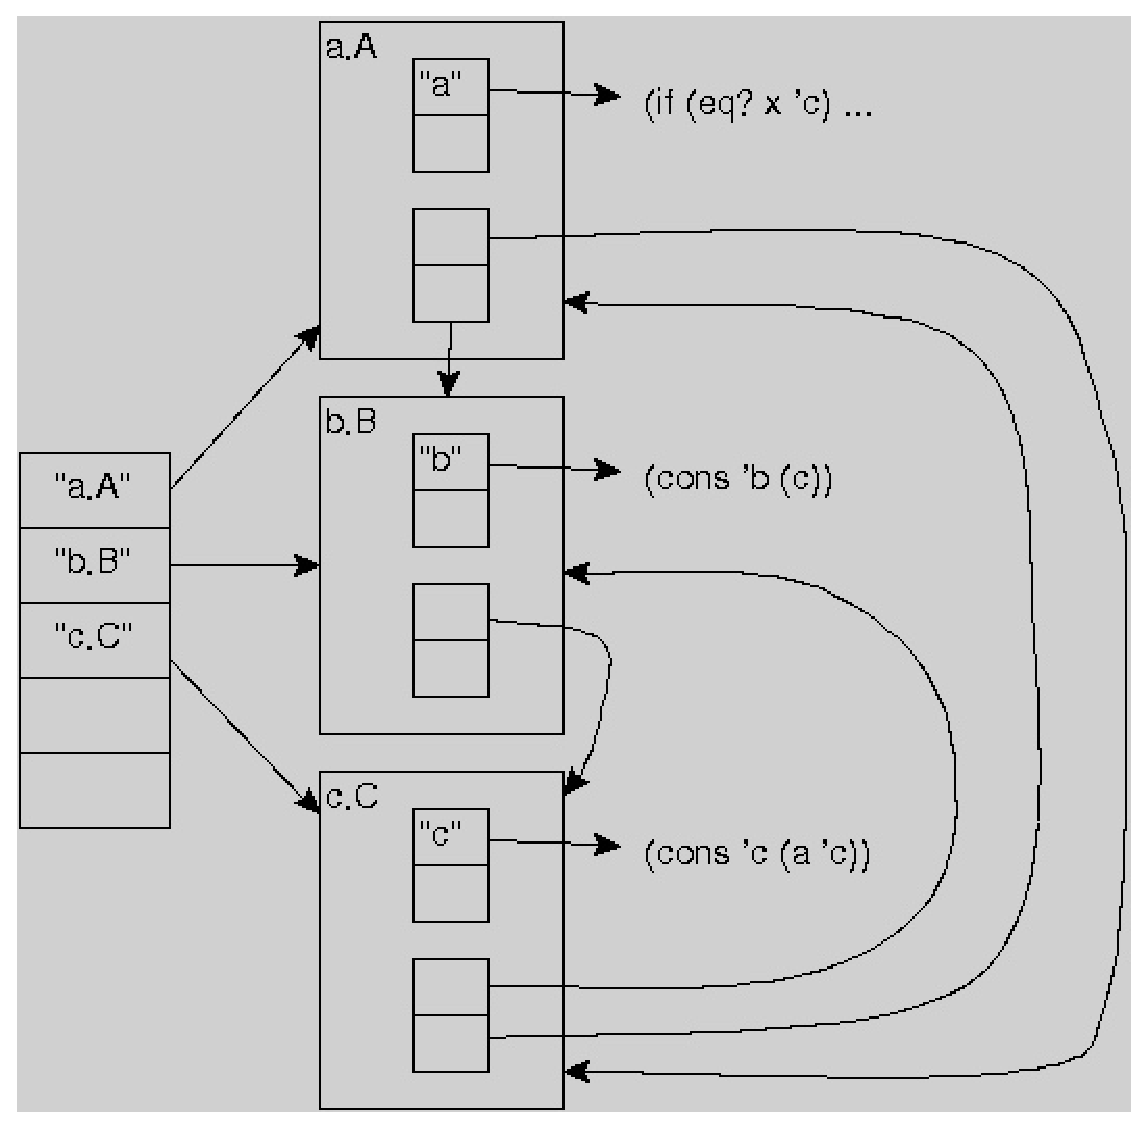
\includegraphics[width=3.1in, height=2.7in]{NamespaceABC}}
\end{picture}
\caption{{\bf Example package structure}}
\label{NamespaceABC}
\end{figure}

The variable binding search algorithm is straightforward: search for
the identifier in the current package's map.  If not found look in the
environment of imported packages.  An optimization is: cache
identifier hash codes and use hash tables that take both the hash code
and the identifier as arguments.  That way the hash code is only
computed once per identifier on demand and each hash table uses the
hash code rather than recompute it.  The identifier is also passed in
to resolve hash conflicts within a hash table.

Although the internal package representation and search algorithm are
straightforward, loading packages is more complex.  Several {\tt
llava} features contribute to the complexity:

\begin{itemize}
\item Java classes can be imported.
\item {\tt llava} provides a REPL, so packages can be defined
on-the-fly interactively and then later become files.
\item A {\tt llava} package file of a package already represented
internally should not be loaded unless it is a new file or has
changed since it was last loaded.
\item Even if a {\tt llava} package file has not been touched it is
still necessary to search the transitive closure of its import list
for any package files that may have changed.
\item Packages can mutually reference each other so load loops must be
detected.
\item New packages automatically import {\tt java.lang.*} and {\tt
org.llava}.
\end{itemize}

When {\tt llava} starts up it creates a {\tt org.llava} package object
for the built-in {\tt llava} procedures (e.g., {\tt eq?}) as shown in
Figure~\ref{NamespaceABCOrgLLava}.  The {\tt org.llava} package object
does not contain any package objects in its imports lists.  Package
objects are also created for {\tt java.lang.*} (the import lists are
left empty).  A package named {\tt llava-} is created as the initial
package for the REPL.  The {\tt llava-} package object contains {\tt
java.lang.*} and {\tt org.llava} in its imports list in that order.
Figure~\ref{NamespaceABCOrgLLava} also shows the result of entering
{\tt (import a.A)} at the REPL.  This causes {\tt a.A} to appear at
the head of {\tt llava-}'s import list and causes a package object to
be created for {\tt a.A}, {\tt b.B} and {\tt c.C} (the later two not
shown).

\begin{figure}[htb]
\unitlength 1in
\begin{picture}(3.1,2.7)(0,0)
\put(0,0){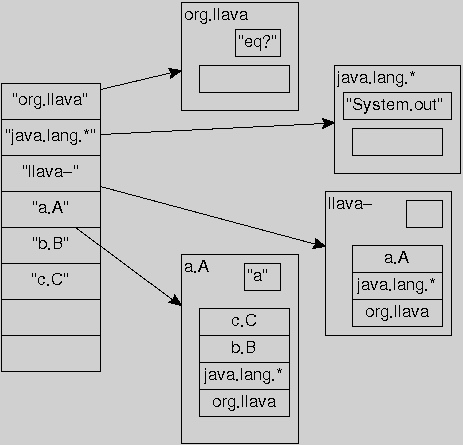
\includegraphics[width=3.1in, height=2.7in]{NamespaceABCOrgLLava}}
\end{picture}
\caption{{\bf llava package structure at startup}}
\label{NamespaceABCOrgLLava}
\end{figure}

\subsubsection{The import algorithm}

The algorithm for importing {\tt llava} files and Java classes into
other packages is shown below.  The discussion assumes the example
packages exist as files.

\small
\begin{verbatim}
if alreadyImportedInPackage?
    loadLlavaFileIfTouched
else existsInPackageNameMap
    addToCurrentPackageImportList
    loadLlavaFileIfTouched
else if java class exists
    import class
    classAlreadyImported = true
    addToCurrentPackageImportList
else
    for path in classpath
        if path/file exists
            load file unless being loaded
            addToCurrentPackageImportList
            break
    if file not found in classpath
        throw FileNotFoundException

\end{verbatim}
\normalsize

\subsubsection{Importing llava files}

When {\tt a.A} is imported it is {\em not} already in the {\tt
llava-} package imports list.
It is {\em not} in the full package name map.
It is {\em not} a Java class file in the classpath.

Therefore search directory and jars on classpath are searched.
When it is found it is loaded.  When {\tt a.A} is loaded the {\tt package}
declaration in its file causes a package object to be created and the
current package to be set to {\tt a.A} while stacking the previous
package (i.e., {\tt llava-}).

For a moment assume {\tt a.A} does not contain {\tt import}
statements.  In that case the rest of {\tt a.A} is read.  That causes
bindings to be entered for top-level variables in the current package
that happens to be {\tt a.A}.  When loading completes the ``package
load stack'' is popped causing the current package to revert back to
{\tt llava-}.  Then the last statement of the import algorithm is
executed causing {\tt a.A} to be pushed onto the front of {\tt
llava-}'s import list.

But {\tt a.A} does contain {\tt import} statements.  When {\tt (import
c.C)} is read while loading {\tt a.A} it causes the import algorithm
to be entered recursively.  Since {\tt c.C} has not been seen before,
all the same steps are taken causing the file for {\tt c.C} to be
loaded.  {\tt c.C}'s package statement causes {\tt c.C} to become the
current package.  Then {\tt (import b.B)} causes the same steps to
occur until the {\tt (import c.C)} inside {\tt b.B} is reached.

At this point the import algorithm detects that {\tt c.C} is in the
process of being loaded so does not load it again.  Then the next
import algorithm step causes {\tt c.C} to be added to {\tt b.B}'s
imports list.  One recursive call of the import algorithm terminates,
and the previous call continues to load {\tt b.B}, causing a procedure
to be bound to variable {\tt b} in {\tt b.B}'s top-level variable map.

When {\tt b.B} finishes loading the next import algorithm step causes
{\tt b.B} to be added to {\tt c.C}'s imports list.  Loading of {\tt
c.C} continues with {\tt c.C}'s next statement {\tt (import a.A)}.
The rest of the transitive loading process follows similar steps.

Figure~\ref{ImportABC} shows the order of loading in this example and
the creation of imports list references.  Dashed arcs indicate that an
imports reference is created but the file is {\em not} loaded since it
is already in the process of being loaded.

\begin{figure}[htb]
\unitlength 1in
\begin{picture}(3.1,2.7)(0,0)
\put(0,0){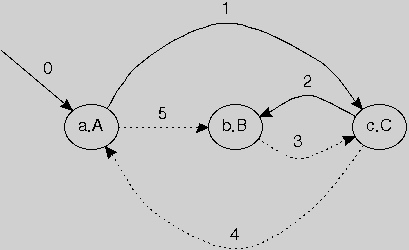
\includegraphics[width=3.1in, height=2.7in]{ImportABC}}
\end{picture}
\caption{{\bf File loading during import}}
\label{ImportABC}
\end{figure}

\subsubsection{Importing a Java class}

When a Java class is imported, {\tt llava} creates a package object
with variables bound to procedures for public constructors, public
static methods and public virtual and static fields in the class.
{\tt llava} does not need to define procedures for public virtual
methods since they are handled automatically by the RI system.  The
imports list of the created package is empty.  The package importing
the Java class has the created package added to its imports list.

\subsubsection{Importing existing packages}

If a package X imports a package Y that is not yet in
the X's import list but Y already has a package object (i.e. {\tt
existsInPackageNameMap} then Y is added to X's imports list.  Further,
if the file has been touched since it was last loaded then load it
again.

The final (top) part of the import algorithm covers the case where package X
imports package Y but Y is already in X's imports list.  In this case
the only thing that needs to happen is loading the package if it has
been touched.

\subsubsection{Loading touched files}

A package being ``touched'' can also mean that a package object exists
for package X because it was created interactively by typing {\tt
(package X)} into the REPL.  At some time later, if a file is created
for package X and if another package imports X, then the file is
loaded.

The algorithm for loading touched files is:

\small
\begin{verbatim}
if not classAlreadyImported
    loop on classpath
        if lastModified = 0 || fileTime > lastModified
            load file
\end{verbatim}
\normalsize

The loading algorithm shows that {\tt llava} does not support
reloading Java classes that have already been imported.  It does
support reloading packages that contain class definitions written in
{\tt llava}.  In that case a new {\tt ClassLoader} is used to contain
the dynamically generated code (discussed later).

When a package is created interactively its package object contains a
{\tt lastModified} field set to 0.  When a file is later found for
that package then the file is loaded and the {\tt lastModified} field
is set to the last modified time of the file.  Later, if the package
is imported again and the file has been touched ({\tt fileTime >
lastModified}) then the file is loaded again.

There are some issues at this point.  When reloading a package that
has been touched should the previous package object be discarded and a
new one created, or should bindings be entered in the existing
package?  If the former (recreating) then any bindings entered in the
REPL are lost.  If the later (use existing) then an erasures are not
seen.  {\tt llava} does recreation.

\subsubsection{Loading reachable touched files}

As discussed, if a package is imported and the file for that package
has not been touched, then it is not loaded again.  However, the
import algorithm (this part is not shown in the pseudo code) loads any
touched files in the transitive closure of the non-touched imported
file.

\subsubsection{Referencing variables by package}

As in Java, {\tt llava} allows references to be short or long.  For
example, {\tt (f)} evaluates to \verb+((c {}) (a {}) (a {}))+ (and
prints {\tt hello}) for the following code:

\scriptsize
\begin{tabular}{l|l}
\verb+(package a.A)+                                   & \verb+(package c.C)+ \\
                                                       &                     \\
\verb+(= h+                                            & \verb+(import a.A)+ \\
\verb+   `(a+                                          & \verb+(import+ \\
\verb+     ,(new 'java.util.Hashtable)))+              & \verb+ java.util.Hashtable)+ \\
                                                       & \verb+(= h+ \\
                                                       & \verb+   `(c+ \\
                                                       & \verb+     ,(new 'Hashtable)))+ \\
                                                       & \verb+(define (f)+ \\
                                                       & \verb+  (list h A.h a.A.h)+ \\
                                                       & \verb+  (println (System.out)+ \\
                                                       & \verb+           "hello"))+ \\
\end{tabular}
\normalsize

In the {\tt llava} implementation, when a variable reference is
executed, if the variable's identifier does not contain dots its value
is searched starting with the current package then continuing with the
imports of that package until found.  If the variable contains dots
then the package part of the identifier is matched against (partial)
package names in the order of the imports list.  Note in the example,
as in Java, that it is not necessary to import a Java class to create
a new instance of that class if the full package and class name is
used.


%==================================================
\subsection{Compiler and runtime system}

The current implementation of {\tt llava} uses two types of
compilation: ``Engine''-based for method bodies and procedure bodies,
and byte code generation for Class definitions.

\subsubsection{Engine-based compilation and execution}

Method and procedure bodies are compiled at read time into instances
of a {\tt Code} class.  There are specific {\tt Code} classes for
application, application args, assignment, if, lambda, literal,
reference, and sequence.  At run time these classes interact with an
{\tt Engine} that enables last-call-optimization.  The {\tt Engine}'s
{\tt run} method interacts with the {\tt run} method on {\tt Code}
instances (simplified):

\small
\begin{verbatim}
public class Engine {
    protected Code code;
    protected ActivationFrame frame;

    public Object run (Code code,
                       ActivationFrame frame) {
        this.code = code;
        this.frame = frame;
        Object result = code.run(frame, this);
        while (result == this) {
            result = this.code.run(this.frame, this);
        }
        return result;
    }
    public Object tailCall (Code code,
                            ActivationFrame frame) {
        this.code = code;
        this.frame = frame;
        return this;
    }
}

public class CodeReference extends Code {
    private int slot;

    public CodeReference (Object source, int slot) {
        super(source);
        this.slot = slot;
    }
    public Object run (ActivationFrame frame,
                       Engine engine) {
        return frame.get(slot);
    }
}

public class CodeIf extends Code {
    protected Code testCode;
    protected Code thenCode;
    protected Code elseCode;

    public CodeIf (Object source, Code testCode,
                   Code thenCode, Code elseCode) {
        super(source);
        this.testCode = testCode;
        this.thenCode = thenCode;
        this.elseCode = elseCode;
    }
    public Object run (ActivationFrame frame,
                       Engine engine) {
        Boolean test = 
            (Boolean) engine.run(testCode, frame);
        if (test.booleanValue() == true) {
            return engine.tailCall(thenCode, frame);
        }
        return engine.tailCall(elseCode, frame);
    }
}
\end{verbatim}
\normalsize

{\tt Code} instances can return a value like {\tt CodeReference}.  In
that case {\tt Engine} detects that the returned value is not the {\tt
Engine} itself and {\tt Engine.run} returns that value.  {\tt Code}
instances can also arrange to have the {\tt Engine.run} method to
continue in its loop evaluating further code by calling {\tt
tailCall}.  {\tt tailCall} sets the {\tt Code} to be executed and the
current activation frame in the {\tt Engine} then returns the {\tt
Engine} itself.  Therefore {\tt Engine.run} will continue its loop.
This engine technique was used in older versions of Jscheme.

\subsubsection{Byte code generation}

{\tt llava} generates byte code for interfaces and classes defined in
{\tt llava} syntax.  {\tt llava} removes method bodies and replaces
them with code to call a procedure representing the body as shown in
Table~\ref{classCompilation}.


\begin{table*}
\caption{Compiling classes}
%\tiny
%\scriptsize
%\footnotesize
%\small
%\normalsize
{\scriptsize

\begin{Parallel}{0.4\textwidth}{0.4\textwidth}

  \ParallelPar
  \ParallelLText{\begin{verbatim}

package org.openhc.llavademo.pb;

import java.util.LinkedList;

import org.llava.F;
import org.llava.Pair;
import org.llava.impl.util.List;

public abstract class PointBase {
    static { 
        F.rce("(import org.openhc.llavademo.pb.PointBase-LLAVA)");
    }

    protected java.util.List history = new LinkedList();
    protected int x = 0;
    protected int y = 0;

    public int getX() {
        Pair app = List.list(F.newSymbol("PointBase-LLAVA-getX"), this);
        return((Integer)F.ce(app)).intValue();
    }
    ...
    protected void move(int dx, int dy) {
        Pair app = List.list(F.newSymbol("PointBase-LLAVA-move"), this,
                             new Integer(dx), new Integer(dy));
        F.ce(app);
    }
    protected void moved() {
        Pair app = List.list(F.newSymbol("PointBase-LLAVA-moved"), this);
        F.ce(app);
    }
    ...
}\end{verbatim}}
  \ParallelRText{\begin{verbatim}
(package org.openhc.llavademo.pb.PointBase-LLAVA);

(define PointBase-LLAVA-getX
  (lambda (this)
    (-f 'x this)))

...
(define PointBase-LLAVA-move 
  (lambda (this dx dy)
    (-f 'x this (+ (-f 'x this) dx))
    (-f 'y this (+ (-f 'y this) dy))
    (moved this)))

(define PointBase-LLAVA-moved
  (lambda (this)
    (add (-f 'history this) (toString this))
    (println (System.out)
	     (+ "Moved: " this))))
...
\end{verbatim}}
\end{Parallel}
}
\label{classCompilation}
\end{table*}

{\tt llava} does not actually produce a textual representation of the
class shell shown in the table.  It generates byte codes for that
shell.  It does create the textual representation of the method bodies
(but does not write them to disk).

After generating the class byte code and {\tt llava} procedures for
method bodies, {\tt llava} loads the procedure code in memory.  This
causes the correct packages and imports lists to be created for the
procedures.

After the procedure packages have been loaded {\tt llava} loads the
byte code into a custom {\tt ClassLoader}.  The {\tt static}
initializer in the class is no longer necessary.  It was used at one
time when {\tt llava} wrote the procedure packages to disk.

When calling methods in the generated code, control is transferred to
the corresponding {\tt llava} procedure.  This is done by creating a
Lisp list of the procedure's identifier followed by the methods
(boxed) arguments.  This list is then given to {\tt F.ce}, that is
shorthand for ``compile-then-evaluate'' ({\tt F} is a static
factory.)

The evaluation part of {\tt F.ce} causes the method's corresponding
procedure to be invoked.  The result of the procedure is the result
of {\tt F.ce}.


%======================================================================
\section{Performance}

This section shows the result of executing {\tt tak} \cite{gabriel} on
an Apple iBook 800MHz G3 with 640MB RAM running OS X 10.3.8 using
Apple's 1.4.2\_05 JRE, build 1.4.2\_05-141.4, with the Java HotSpot(TM)
Client VM (build 1.4.2-38, mixed mode).


The JRE was started with {\tt -XX:CompileThreshold=2} to cause the
HotSpot compiler to start early.  The tests were run with 100
``warmup'' loops to ensure all code is loaded and HotSpot compiled.
The times are the average running the test 200 times (after warmup).

Figure~\ref{tak} shows {\tt tak} execution times for Kawa, Jscheme and
{\tt llava}.  In this test, {\tt tak} is defined with an explicit {\tt
lambda} to keep {\tt llava} from entering its RI system.  Therefore
the measurements are of Scheme procedure calls.  Both Jscheme and {\tt
llava} are an order of magnitude slower than Kawa, indicating those
systems could benefit from byte code generation of procedure bodies.

\begin{figure}[htb]
\unitlength 1in
\begin{picture}(3.1,2.7)(0,0)
\put(0,0){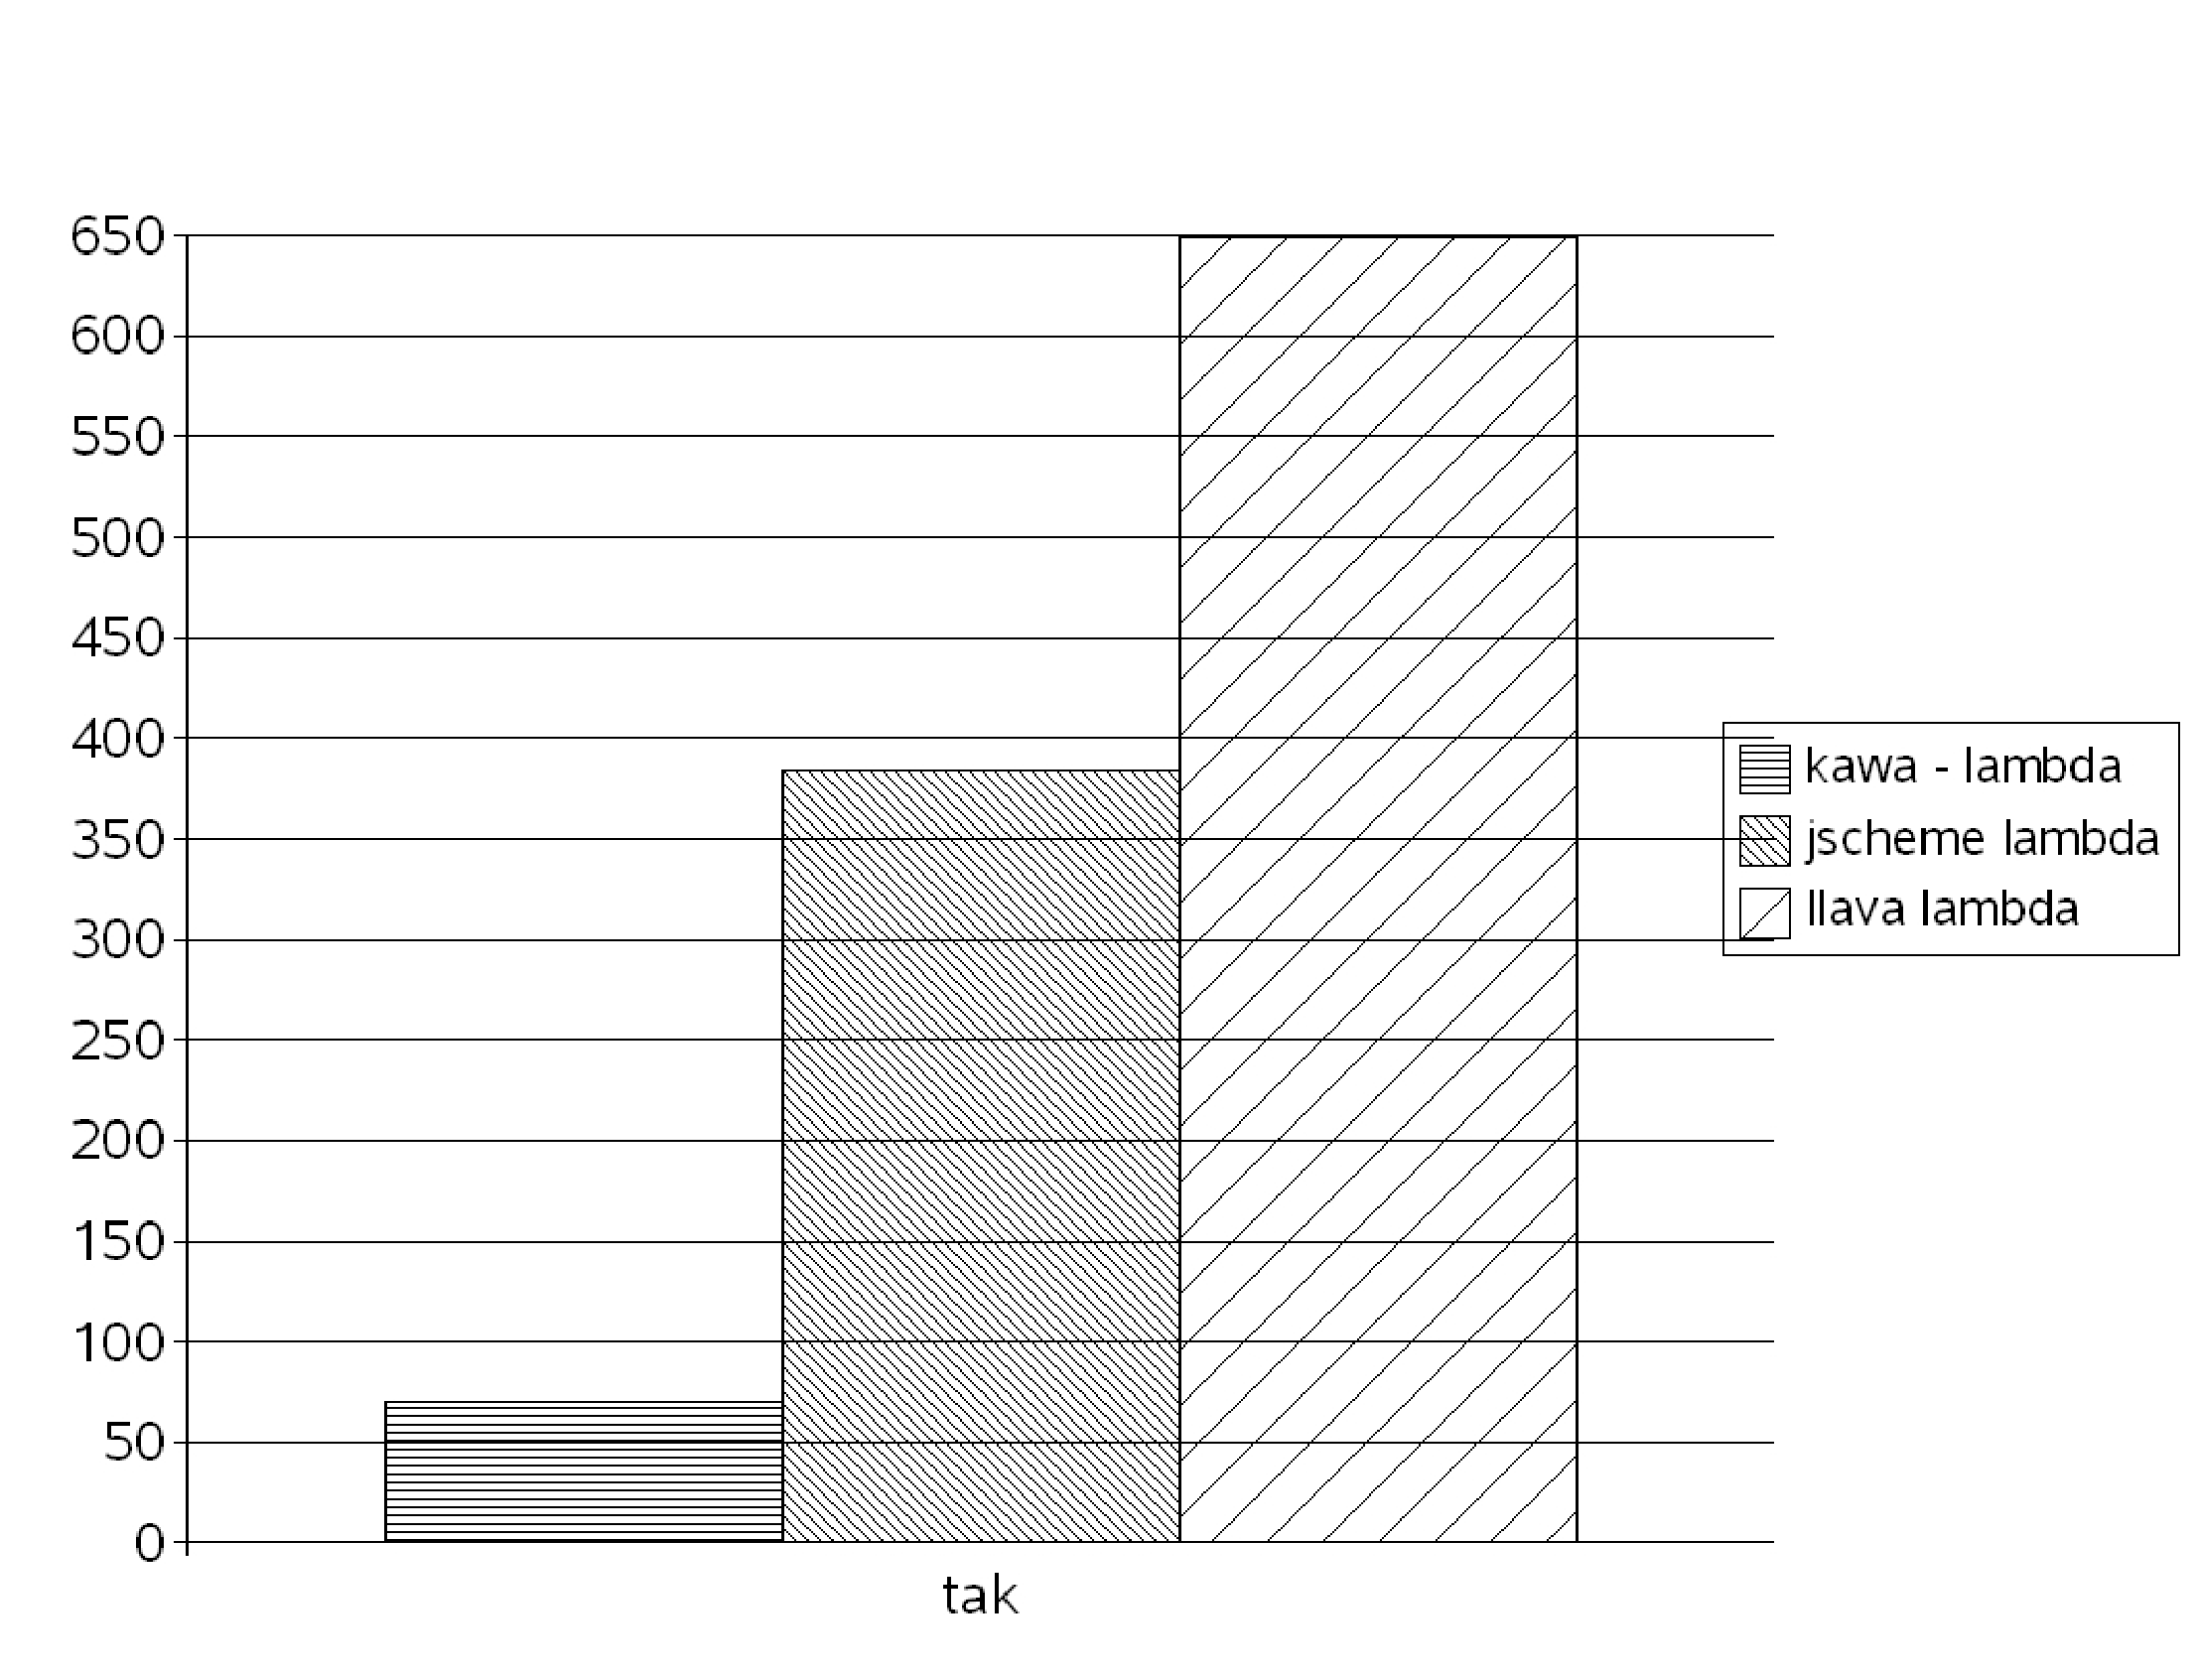
\includegraphics[width=3.1in, height=2.7in]{tak}}
\end{picture}
\caption{{\bf Tak time}}
\label{tak}
\end{figure}

Figure~\ref{takRiLambda} shows the {\tt llava} execution time of {\tt
tak} defined with an explicit {\tt lambda} compared to a generic
(i.e., RI) definition.  This means the comparison is between direct
procedure calls and the cost of trying and failing reflection.  It is
clear that the overhead is large.  No time has been spent optimizing
any part of {\tt llava} so improvements are possible.  In particular,
RI indicates failure by throwing exceptions.  It would be better to
{\em return} ``failure objects.''  As a quick experiment, parts of RI
were rewritten to return failure objects.  This resulted in the time
shown in the third column labeled ``llava RI opt.''


\begin{figure}[htb]
\unitlength 1in
\begin{picture}(3.1,2.7)(0,0)
\put(0,0){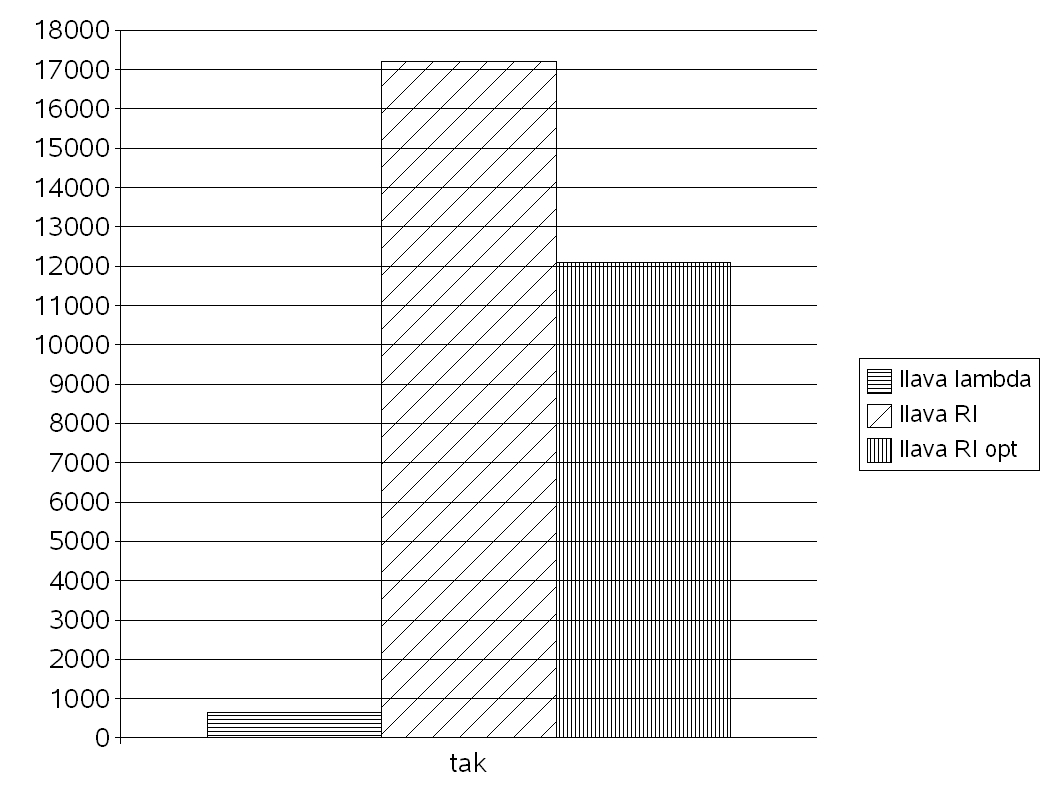
\includegraphics[width=3.1in, height=2.7in]{takRiLambda}}
\end{picture}
\caption{{\bf llava tak lambda/RI time}}
\label{takRiLambda}
\end{figure}


Figure~\ref{fprintRead} show Kawa, Jscheme and {\tt llava} times for
the {\tt fprint} and {\tt fread} benchmarks \cite{gabriel}.  These
times increase our confidence in the accuracy of the {\tt tak} times
since it is expected that these times be similar since all three
systems implement Scheme {\tt read} and {\tt write} in Java (therefore
time spent in the evaluators is minimal).


\begin{figure}[htb]
\unitlength 1in
\begin{picture}(3.1,2.7)(0,0)
\put(0,0){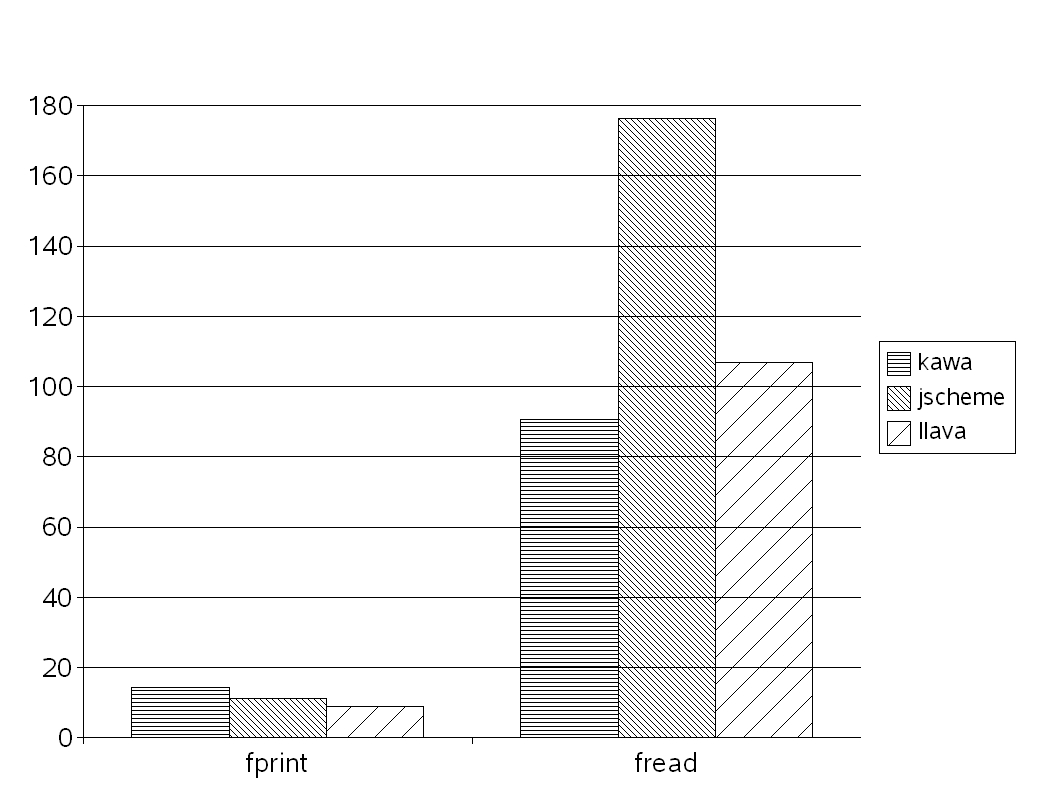
\includegraphics[width=3.1in, height=2.7in]{fprintRead}}
\end{picture}
\caption{{\bf fprint/fread time}}
\label{fprintRead}
\end{figure}



%======================================================================
\section{Conclusions and Future Work}

{\tt llava} is an idea and an implementation.  It is clear that the
implementation needs improvement.  But, more important at this time,
is the idea: Java in Lisp syntax extended with procedures and macros.
{\tt llava} brings the Lisp's adaptability to Java.

The main future work is continued {\tt llava} language design to bring
it on par with Java 5.  Of course, even if and when Java 5 parity is
reached, {\tt llava} language design is unending as Java continues to
evolve.

Much implementation work remains.  The current implementation of {\tt
llava} works on JDK 2.0 and above.  The implementation could benefit
from Java 5 features and speed.  It is clear from the performance
figures that the implementation can use extensive optimizations or
alternatives.

The RI need optimization.  The first, already mentioned, is to report
failure by {\tt return} rather than by {\tt throw}.  Better caching of
previously found methods could improve performance.

The Engine-based compiler and runtime system could be replaced by byte
code generation.  Once that is done then {\tt llava}'s current class
compilation technique can be replaced with direct compilation of the
method bodies inline.  

The {\tt llava} implementation has been written such
that multiple versions of {\tt llava} can exist independently in the
same VM.  However, the existing class compilation technique relies on the
existence of a ``global'' static variable to gain access to the {\tt
llava} system.  This should be avoided.

Despite the implementation's shortcomings, the idea of {\tt llava} is
clear: Java in Lisp syntax.  {\tt llava} brings the advantages of Lisp
to Java in a natural intuitive representation.


%======================================================================
\section{Acknowledgments}

Thanks to Per Bothner, Michael Travers, Peter Norvig, Ken Anderson and
Tim Hickey for their implementations of Scheme in Java.  {\tt llava}
uses ideas or implementation techniques from their systems.  Thanks to
Ken Cavanaugh and Tim Hickey for their comments on the final draft of
this paper.  And thanks to Gilad Bracha for encouragement.



%%%%%%%%%%%%%%%%%%%%%%%%%%%%%%%%%%%%%%%%%%%%%%%%%%%%%%%%%%%%%%%%%%%%%%%%%%%%%%
\begin{thebibliography}{1}

\bibitem{LaSC5} R.~Kessler, H.~Carr, L.~Stoller, and M.~Swanson.
\newblock Implementing Concurrent Scheme for the Mayfly distributed
parallel processing system.  \newblock {\em Lisp and Symbolic
Computation}, Vol 5, Issue 1-2 (May 1992) pp 73-93.
%http://portal.acm.org/citation.cfm?id=161270.161285&dl=GUIDE&dl=GUIDE&CFID=33708534&CFTOKEN=68233485

\bibitem{LaSC3}
P.~Pourheidari, R.~Kessler, and H.~Carr.
\newblock Moped (a portable debugger)
\newblock {\em Lisp and Symbolic Computation}, Vol 3, Issue 1 (January 1990) pp 39-65.
%http://portal.acm.org/citation.cfm?id=83661.83679&coll=GUIDE&dl=GUIDE&CFID=33708534&CFTOKEN=68233485

\bibitem{DC++}
H.~Carr, R.~Kessler, and M.~Swanson.
\newblock Distributed C++
\newblock {\em ACM SIGPLAN Notices}, Vol 28, Issue 1 (January 1993)
%http://portal.acm.org/citation.cfm?id=156702&jmp=indexterms&dl=GUIDE&dl=GUIDE

\bibitem{kawa}
Per Bothner
\newblock kawa
\newblock http://www.gnu.org/software/kawa/

\bibitem{JschemeDot}
K.~Anderson, T~.J.~Hickey, P.~Norvig
\newblock Silk: A Playful Combination of Scheme and Java
\newblock {\em Proceedings of the Workshop on Scheme and Function Programming} , pp 13-22
\newblock Rice University, CS Dept. Technical Report 00-368, September 2000.
\newblock http://www.cs.brandeis.edu/~tim/Papers/Reflection99/ silk2000.pdf

\bibitem{abcl}
\newblock ArmedBear Common Lisp
\newblock http://armedbear-j.sourceforge.net/


\bibitem{JschemeEngine}
T.~J.~Hickey, P.~Norvig, K.~Anderson
\newblock LISP - a Language for Internet Scripting and Programming
\newblock in LUGM'98: The 40th Anniversary of LISP: Lisp in the Mainstream, Nov. 1998, Berkeley, CA.
\newblock http://www.cs.brandeis.edu/~tim/Papers/Reflection99/ lugm.ps

\bibitem{queinnec}
C.~Queinnec
\newblock {\em Lisp in Small Pieces}
\newblock Cambridge University Press, 1996

\bibitem{skij1}
T.~Travers
\newblock Skij
\newblock http://xenia.media.mit.edu/~mt/skij/

\bibitem{skij2}
T.~Travers
\newblock Scripting and Dynamic Interaction in Java
\newblock http://xenia.media.mit.edu/~mt/skij/dynjava/ dynjava.html

\bibitem{skij3}
T.~Travers
\newblock Dynamic Interaction in Java
\newblock Dr. Dobb's Journal (25:1) January 2000
\newblock http://www.ddj.com/documents/s=889/ddj0001l/ 0001l.htm

\bibitem{JschemeReflection}
K.~Anderson, T.~J.~Hickey,
\newblock Reflecting Java Through Scheme
\newblock {\em Proceedings of the Second International Conference on Metalevel Architectures and Reflection}
\newblock Springer-Verlag Lecture Notes in Computer Science, vol. 1616, pp. 154-174, 1999.
\newblock (Reflection'99), Saint-Malo, France, July 19-21,1999

\bibitem{gabriel}
R.~P.~Gabriel
\newblock {\em Performance and Evaluation of Lisp Systems}
\newblock MIT Press Series in Computer Science, MIT Press, Cambridge, MA, 1985
\newblock http://www.dreamsongs.com/NewFiles/Timrep.pdf

\end{thebibliography}

\end{document}

% End of file.



